
% tipo de documento
\documentclass{article}

% formato de página
\usepackage[margin=1.5cm, letterpaper]{geometry}

% idioma de los macros
\usepackage[spanish]{babel}
\usepackage[utf8]{inputenc}

% vínculos
\usepackage{hyperref}

% manejo de ecuaciones
\usepackage{amsmath}

% manejo de figuras
\usepackage{graphicx}
\usepackage{float}

% texto del documento
\begin{document}
    \title{
        Organización y Arquitectura de Computadoras \\
        Práctica 6: Lenguaje ensamblador \\
    }
    \date{
        31 de marzo del 2019
    }
    \author{
        Sandra del Mar Soto Corderi \\
        Edgar Quiroz Castañeda
    }
    \maketitle

    \section{Preguntas}
    \begin{enumerate}
    	%1.
        \item {
        	A partir del ejercicio 4:
            \[4\cdot\sum_{n=0}^{m}{\frac{(-1)^{n}}{2n+1}}\]
            \begin{enumerate}
            	%a)
                \item ¿A qué valor tiende la serie?\\
                Es la fórmula de Leibniz\cite{wolfram pi} para aproximar $\pi$.\\
                
                %b)
                \item ¿A cuántos dígitos se puede aproximar ese valor?\\
                Como es precisión sencilla, se pueden aproximar hasta 23 bits
                del valor en binario, que equivalen a 7 dígitos de precisión en
                decimal\cite{ieee flot32 std}.\\
                
                %c)
                \item ¿Cuántas iteraciones son necesarias para llegar a esa
                aproximación? \\
                Los primeros 7 dígitos de $\pi$ son 3.141592\cite{pi dig}. Se puede llegar a esta aproximación con 250000 iteraciones.
                \begin{figure}[H]
                    \centering
                    \caption{Resultado de las aproximaciones}
                    \label{appVal}
                    \begin{tabular}{|l|l|}
                        \hline
                        Iteraciones & Aproximación \\ \hline
                        50000       & 3.1415758    \\ \hline
                        10000       & 3.1415758    \\ \hline
                        250000      & 3.141592     \\ \hline
                        500000      & 3.141594     \\ \hline
                        1000000     & 3.1415954    \\ \hline
                        3000000     & 3.1415963    \\ \hline
                        4000000     & 3.1415966    \\ \hline
                        5000000     & 3.1415966      \\ \hline
                    \end{tabular}
                \end{figure}
                \begin{figure}[H]
                    \centering
                    \caption{Error por iteraciones al intentar aproximar 3.141592}
                    \label{err}
                    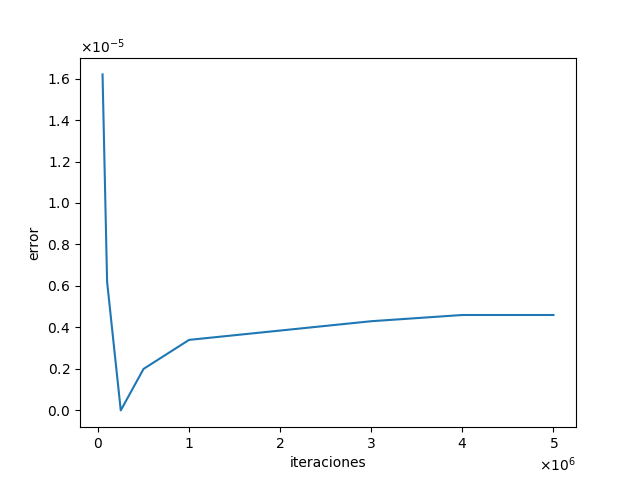
\includegraphics[scale=0.5]{python/error.png}
                \end{figure} 
            	El programa con el cual se elaboró la gráfica se encuentra dentro de la carpeta python.\\
            	           
                Se puede apreciar en \eqref{err} que se llega a un error de 0 en
                250,000 iteraciones. Tanto antes como después de ese punto, la
                aproximación empeora entre más se aleja de ese número.\\
                Esto es de esperarse para iteraciones menores a 250,000, pero 
                es inusual para valores mayores, pues entre mayor sea $m$ el valor
                de la serie calculada debería ser más cercana al valor de la 
                serie infinita.\\
                Este error puede deberse a que al ser el $m$ grande, el término
                $\frac{1}{2n+1}$ se vuelve más pequeño, por lo que el error en su representación en punto flotante 32 bits puede aumentar.
                Así, la aproximación empeora.\\
            \end{enumerate}
        }
    	%2.
        \item ¿Existe alguna diferencia en escribir programas en lenguaje 
        ensamblador comparado con escribir programas en lenguajes de alto nivel?\\
        Escribir programas de alto nivel permite abstraer e implementar conceptos
        sin necesidad de tener en cuenta la traducción a código máquina, lo que hace que se pueda ignorar toda la parte física de la computadora. Además la mayoría de lenguajes de alto nivel proporcionan grandes bibliotecas que manejan tareas como entrada/salida, conversiones numéricas, y operaciones de encadenamiento.  Mientras que la mayoría de los sistemas de desarrollo en lenguaje ensamblador, le dejan la responsabilidad al programador de proporcionar esta funcionalidad para sus aplicaciones.
        
        %3.
        \item ¿En qué casos es preferible escribir programas en lenguaje 
        ensamblador y en qué casos es preferible hacerlo con un lenguaje de alto nivel?\\
        Como depende de la arquitectura de la computadora, el código en lenguaje
        ensamblador no es portable, además de que requiere conocimiento de la
        máquina particular con la se está trabajando. Sin embargo, el código
        producido es de los más eficaces posible.\\
        Entonces, se debería usar ensamblador cuando se esté diseñando código
        específico de hardware que requiere ser muy eficaz, como lo requieren
        algunos compiladores o ciertos fragmentos de sistemas operativos. Y utilizar lenguajes de alto nivel en programas más complejos y que se utilicen en arquitecturas distintas de hardware.
        
    \end{enumerate}

    \begin{thebibliography}{1}
        \bibitem{ieee flot32 std} 
        \textit{IEEE Standard for Floating-Point Arithmetic},
        IEEE Std 754-2008, 2008. [Online]. Disponible: 
        \url{https://ieeexplore.ieee.org/document/4610935}.
        [Consultado: 28-Mar-2019].
        
        \bibitem{wolfram pi}
        E. W. Weisstein, \textit{Pi Formulas}, Wolfram MathWorld. [Online]. 
        Disponible: \url{http://mathworld.wolfram.com/PiFormulas.html}.
        [Consultado: 28-Mar-2019].

        \bibitem{pi dig}
        M. Huberty, K. Hayashi and C. Vang, \textit{100,000 Digits of Pi}, 
        Geom.uiuc.edu, 1997. [Online]. Disponible: 
        \url{http://www.geom.uiuc.edu/~huberty/math5337/groupe/digits.html}. 
        [Consultado: 28-Mar-2019]
    \end{thebibliography}
\end{document}